\begin{chapter}{\label{cha:afm}Simulating the rough surface of a ``Floppy Wire''}
\section{Introduction}
At sufficiently low temperatures, liquid helium has two striking
properties.  Firstly, it flows without viscosity.  Secondly,
its vorticity is constrained to
thin mini-tornadoes, characterised by their fixed circulation
$h/m$ (the ratio of Planck's constant to
the mass of the relevant boson - one atom in $^4$He and one Cooper pair 
in $^3$He-B) and microscopic core radius $\xi$ 
($0.1~\rm nm$ in $^4$He and $10~\rm nm$ in $^3$He-B).  
In contrast, the eddies in everyday viscous fluids can have arbitrary shape, 
size and circulation.  

Of ongoing experimental and theoretical study is the nature of 
turbulence in superfluids 
\cite{Barenghi2014,Bradley11,PhysRevLett.115.155303,PhysRevLett.110.014502}, a state 
dominated by an irregular tangle of quantised vortex lines.  Despite the fundamental differences between superfluids and classical fluids, the observations of Kolmogorov energy spectra, famed from classical isotropic turbulence, in superfluid turbulence \cite{Barenghi2014} are suggestive of a deep connection between them.  Superfluid turbulence is nowadays most commonly formed by moving obstacles, including grids \cite{Davis2000}, wires \cite{Guenault1986,Bradley2005,Bradley2011,Fisher2001}, forks \cite{Blaauwgeers2007,Bradley2012}, propellers \cite{Tabeling1998,Salort}, spheres \cite{Schoepe1995} and other objects \cite{VinenSkrbek2008}.
Despite progress in visualizing the flow of superfluid helium in the
bulk \cite{PhysRevLett.115.155303,PhysRevB.92.064519}, including individual vortex reconnections
\cite{Bewley09}, there is little direct experimental evidence
about what happens at boundaries.
Here, vortices are believed to be generated by two mechanisms.  Firstly, 
they can nucleate at the boundary of the vessel or object.  
When the relative flow speed is sufficiently low, the flow is laminar 
{(potential)} and dissipationless.  
{Near curved boundaries, however, vortex nucleation occurs if
the local flow velocity exceeds a critical value.} 
Secondly, the vortices can be procreated from so-called `remnant vortices' 
which are present in the system since cooling the helium through the superfluid transition.  Note that remnant vortices can be avoided using judicious, slow experimental protocols \cite{PhysRevB.76.020504}. 

The nano-scale vortex core in superfluid helium is comparable in size 
to the typical roughness of the boundaries of the vessel or stirring object. 
Unfortunately the lack of direct experimental information about vortex 
nucleation at the boundaries and the subsequent vortex-boundary interactions,
limit the interpretation of experiments. Theoretical
progress is challenging and to date has focussed on smooth and idealised surfaces.  In principle, the superfluid boundary conditions
are straightforward:
the superfluid velocity
component which is perpendicular to the boundary must vanish
at the boundary, whereas the tangential component (in the absence of
viscous stresses) can slip.  For the latter reason, we do not expect boundary layers,
typical of viscous flows.   
Implementing these {superfluid} boundary conditions, 
Schwarz \cite{Schwarz-bump}
and Tsubota {\it et al.} \cite{PhysRevB.50.579}
found that one or more vortices sliding along a smooth surface
can become deflected or trapped by a small
hemispherical bump.  Such bumps can also serve as nucleation sites for vortices;  the local superfluid velocity is raised at the pole of the bump and more readily breaks the critical velocity for vortex nucleation \cite{win01}.  Moreover, recent simulations \cite{stagg_parker_14} show that, if
the bump is elliptically shaped and elongated perpendicular to the imposed flow, the superfluid velocity at the pole
is enhanced, reducing the critical velocity for vortex nucleation and increasing the vortex nucleation rate (for a given super-critical imposed flow). 
We expect therefore that microscopically-small surface roughness may promote the nucleation of vortices at a surface.
For pre-existing vortex lines in the vicinity of the surface, there is also indirect experimental evidence of a `vortex mill' mechanism 
which continuously feeds vorticity into the flow by stretching 
{the existing vortex} lines. This mechanism only works if the spooling vortex, 
held by pinning sites at the surface, is aligned in the streamwise direction \cite{PhysRevLett.64.1130}.

\section{Method\label{section:methodafm}}
To shed light on the microscopic behaviour of superflow near a rough
boundary, we work with the three-dimensional profile of a real surface, shown in Figure \ref{fig:afmreal}.  This corresponds to a one square micron region of the surface of a thin NbTi wire used to generate quantum turbulence at Lancaster University, as profiled via atomic force microscopy (AFM) \cite{Lawson}.  The surface is rough, with a height up to around 15 nm, and features sharp grooves and steep ridges, likely to have arisen during the etching phase of the wire preparation. We assume that such feature are typical of the wires and similar objects used across other superfluid turbulence experiments. 

\begin{figure}
  \centering
  \begin{tikzpicture}
    \begin{axis}[
        width=0.5\linewidth,
        xlabel={$x$ ($\mu$m)},
        ylabel={$y$ ($\mu$m)},
        xmin=-0.5,
        xmax=0.5,
        ymin=-0.5,
        ymax=0.5,
        major tick length = 0.07cm,
        axis on top,
        unit vector ratio=1 1 1,
        axis on top,
        colorbar style={title={\makebox[\linewidth]{Height (nm)}},text width=0.5em,major tick length = 0.07cm},
        major tick length = 0.07cm,
        point meta min = 0,
        point meta max = 16,
        colorbar,colormap/jet
      ]
      \addplot graphics [xmin=-0.5,xmax=0.5,ymin=-0.5,ymax=0.5] {afm/afm2.png};
    \end{axis}
  \end{tikzpicture}
  \caption{\label{fig:afmreal}AFM image of a section of the NbTi wire used to generate turbulence in superfluid helium at Lancaster University (data provided by R. P. Haley and C. Lawson).}
\end{figure}

Traditionally, the Vortex Filament Model (VFM) \cite{Schwarz}
has been used to model the motion of vortex lines in the presence of
smooth spherical \cite{Hanninen-sphere,Kivotides-sphere},
hemispherical \cite{Schwarz-bump,PhysRevB.50.579} 
and cylindrical boundaries \cite{Hanninen-PNAS,goto08}.
However the model is unsuitable for our purposes for several reasons.
Firstly, it assumes that the vortex core is infinitesimal compared to 
any other length scale, which is not the case if
vortex core and wall roughness are comparable.
Secondly, microscopic behaviours such as vortex nucleation or kinetic energy losses due
to sound emission are not captured. For example, VFM requires the arbitrary seeding of
vortex loops in order to generate turbulence.
Thirdly, it is difficult to generalise from smooth, geometrically simple (cylindrical or spherical)
boundaries to the rough boundaries which interest us.

Another approach which suffers similar difficulties \cite{Henderson} is
the two--fluid Hall--Vinen--Bekarevich--Khalatnikov (HVBK)
equations \cite{Salort2011,Salort2012}. Moreover, the HVBK equations are coarse--grained over
length scales larger than the average vortex separation, hence the
boundary conditions require further assumptions or the introduction of
unknown sliding/pinning parameters.


We instead model the flow of superfluid helium over this surface through the Gross-Pitaevskii equation (GPE) \cite{RobertsBerloff} for a weakly-interacting Bose superfluid, as described in Chapter \ref{cha:theoretical_model}. The GPE is equivalent to a hydrodynamic model with fluid density $n({\bf r},t)=|\psi({\bf r},t)|^2$ and velocity ${\bf v}({\bf r},t)=(\hbar/m)\nabla \theta$, and embodies a classical 
continuity equation and a modified Euler equation (the modification being the presence of a quantum pressure term, arising from zero-point motion of the particles {and responsible for vortex nucleation}). Further details of the hydrodynamic description of the GPE can be found in Section \ref{section:hydrodynamic}.
While the GPE provides only a qualitative model of the strongly-interacting superfluid helium (for example, the excitation spectrum of the GPE lacks helium's roton minimum), it nevertheless contains the key microscopic physical ingredients of our problem: finite-size vortex core, vortex interactions and vortex reconnections \cite{RobertsBerloff}.  Furthermore, any boundary, however irregular, can be conveniently modelled through the potential $V({\bf r},t)$. The GPE modelled is numerically simulated in the the homogeneous form as described in Section \ref{section:gpedimlesshomg}, and so in this chapter we report quantities scaled in the natural units: the vortex core size is characterised by the healing length $\xi=\hbar/\sqrt{m \rho g}$ and the natural speed, energy and time scales are provided by the speed of sound $c=\sqrt{\rho g/m}$, the chemical potential $\mu=\rho g$ and the unit $\tau=\xi/c$, respectively. 

\begin{figure}
  \centering
  \begin{tikzpicture}
    \begin{axis}[
        width=0.5\linewidth,
        xlabel={$x/\xi$},
        ylabel={$y/\xi$)},
        xmin=-200,
        xmax=200,
        ymin=-200,
        ymax=200,
        major tick length = 0.07cm,
        axis on top,
        unit vector ratio=1 1 1,
        axis on top,
        colorbar style={title={\makebox[\linewidth]{$z/\xi$}},text width=0.5em,major tick length = 0.07cm},
        major tick length = 0.07cm,
        point meta min = 0,
        point meta max = 105,
        colorbar,colormap/jet
      ]
      \addplot graphics [xmin=-200,xmax=200,ymin=-200,ymax=200] {afm/afmsmoothn.png};
      \addplot+[mark=none,color=black,ultra thick,dashed] [domain=-205:205] {0*x+20};
    \end{axis}
  \end{tikzpicture}
  \caption{\label{fig:afmsmooth}AFM image of a section of the NbTi wire rough surface, mapped into the computational coordinate system and smoothed by a Gaussian blur (standard deviation 6 nm) so as to remove discontinuities in the surface profile. The profile used in our 2D simulations ($y=0.05\,\mu$m) is marked by a dashed line.}
\end{figure}

Our results are based on intensive simulations of the GPE over the entire AFM surface, resolved down to a sub-core scale of $\Delta=0.4\xi$. In $^4$He the vortex core size is $a_0 \approx 10^{-10}~\rm m$ \cite{Rayfield1964}, such that the AFM image has true core dimensions $(10^4 \times 10^4 \times 100) a_0^3$.  It is not computationally feasible to model the corresponding range of scales directly within the GPE; as such we map the AFM image onto the largest practical healing length volume of $(400 \times 400 \times 100) \xi^3$.  This is simulated in a box of size $(400 \times 400 \times 200) \xi^3$ (the numerical domain being twice as high as the highest point of the data in the third dimension), on a $1000\times 1000\times 500$ spatial grid, which is periodic in $x$ and $y$.  We smooth the original AFM data with a Gaussian blur (standard deviation 6 nm), so as to remove discontinuities in the surface profile, as shown in Figure \ref{fig:afmsmooth}. The rough surface is then incorporated into the GPE by setting a potential barrier $V=5\mu$ below the surface, heavily prohibiting density there; above the surface the density recovers to the bulk value $n_0$ (where $V=0$) over a length scale of the order of $\xi$. Section \ref{section:3dafmpotential} describes the form of $V$ in detail. Additionally, in all our simulations the zero level of the $z$ dimension is arbitrarily shifted so that the minimum height of the two or three-dimensional surface profile is fixed at $z=0$, so as to optimise use of the computational box. Time evolution is performed with the 4th order Runge-Kutta scheme described in Section \ref{section:RK4} with time step $\Delta t=0.01 \tau $, and performed across 256 (2.6 GHz) cores of a high-performance {computer} cluster.

Our simulations of in 3D model the entire rough surface by using the entire AFM data as a 3D potential. However, in the interests of effective exploration of the parameter space, we also perform some reduced simulations in two dimensions. Here we simulate only a single row of the AFM data (marked in Figure \ref{fig:afmsmooth} and shown in detail in Figure \ref{fig:surfprofile}) using the 2D GPE, ignoring the $y$ dimension. The selected row was chosen so as to contain a two-dimensional analogue of the steep ridge structures exhibited along the wire's surface.

We first obtain the stationary solution of the GPE in the presence of
the rough boundary, with bulk density $\rho$.  The GPE is then transformed into a frame moving at speed $u$ in the negative $x$-direction (corresponding to the imposed flow) by the addition of a Galilean boost term $ i \hbar u \partial \Psi/\partial x$ to the right-hand side of the GPE, as described in Section \ref{section:linearmovframe}.  The flow speed is ramped up smoothly from zero to the final value of $u=0.2\,c$ in one simulation, and $u=0.6\,c$ in another; these final values are such that the critical velocity for nucleation is exceeded. 

\section{Two-dimensional results}
\begin{figure}
  \centering
  \begin{tikzpicture}
    \begin{axis}[
        width=0.7\linewidth,
        xlabel={$x/\xi$},
        ylabel={$y/\xi$},
        xmin=-200,
        xmax=200,
        ymin=0,
        ymax=60,
        unit vector ratio=1 1 1,
        major tick length = 0.07cm,
        axis on top,
        major tick length = 0.07cm
      ]
      \addplot graphics [xmin=-200,xmax=200,ymin=0,ymax=60] {afm/afmside.png};
    \end{axis}
  \end{tikzpicture}
  \caption{\label{fig:surfprofile} The 2D rough surface profile that we employ in our two-dimensional simulations. The surface is taken from the full AFM data so as to capture one of the `mountain' features present on the surface. The data is mapped onto our computational coordinate system as described in Section \ref{section:methodafm} and the exact mapping is shown here.}
\end{figure}

We begin by focusing on our two-dimensional simulations. For the surface depicted in Figure \ref{fig:surfprofile}, we find the critical velocity for vortex nucleation to be $v_c=(0.125\pm0.025)\,c$. This is significantly less than the critical velocity for a circular obstacle (which has a critical velocity of $v_c\approx 0.38\,c$ \cite{frisch92,nore93,win00,huepe00}). This result shows that the effect described throughout Chapter \ref{cha:wake} is also occurring for the peak of the elliptical-like feature extruding from the surface. The location acts as a nucleation site due to the high curvature which induces a high local fluid velocity, and so landau's criterion is broken here before anywhere else in the system. We will call such structures in the surface of the wire that induce this property `mountains'.

\subsection{Vortex nucleation}
\subsubsection{Early-time vortex nucleation}
At early times the resulting flow depends on the velocity of the imposed fluid flow. Below the critical velocity, the fluid undergoes smooth potential flow around the surface. The instantaneous streamlines of this flow, demonstrated in Figure \ref{fig:earlyvsv}(a), vary smoothly around the surface with streamlines far away from the surface straight and unaffected by the roughness, and streamlines near the surface showing high curvature.

At velocities above the the critical velocity, a series of vortices nucleate from the peak of the highest mountain. We call this the primary nucleation site. The circulation of the vortices produced in the wake of the mountain will depend on the direction of the imposed flow. In our simulations the flow is in the negative $x$ direction and so the produced vortices have positive circulation.

The strength of the imposed flow affects the vortex nucleation frequency, so that for larger flow velocities more vortices are produced in a given time period. This is confirmed for the case of this surface, and modified surfaces, by measurement of $N_v$ at different flow velocites, shown in Table \ref{tbl:nv_bl}. For velocities just higher than the critical velocity, vortices nucleate from the mountain at low enough frequency that the fall downstream and do not interact significantly. For high velocities, however, many vortices nucleate in close proximity and interact strongly with one another. Vortex co-rotation is induced and this leads to the vortices combining into a larger-scale cluster of positive circulation. Figure \ref{fig:earlyvsv} shows the early post-nucleation configuration for different imposed flow speeds. 

\begin{figure}
  \centering
  \makebox[\textwidth]{%
  \begin{minipage}{1.1\textwidth}%
  \hspace{0.5cm}(a) \hspace{5cm}(b) \hspace{4.75cm}(c)\\
    \begin{tikzpicture}%
    \begin{axis}[
      width=0.35\linewidth,
      xlabel={$x/\xi$},
      ylabel={$y/\xi$},
      xmin=-200,
      xmax=200,
      ymin=0,
      ymax=200,
      unit vector ratio=1 1 1,
      major tick length = 0.07cm,
      axis on top
    ]
    \addplot graphics [xmin=-200,xmax=200,ymin=0,ymax=200] {afm/stream};
    %\addplot+[mark=none,blue,style=solid] file {afm/streams2.dat};
    \addplot+[mark=none,black,style=solid] file {afm/streams3.dat};
    \addplot+[mark=none,black,style=solid] file {afm/streams4.dat};
    \addplot+[mark=none,black,style=solid] file {afm/streams5.dat};
    \addplot+[mark=none,black,style=solid] file {afm/streams6.dat};
    \addplot+[mark=none,black,style=solid] file {afm/streams7.dat};
    \addplot+[mark=none,black,style=solid] file {afm/streams8.dat};
    %\addplot+[mark=none,black,style=solid] file {afm/streams9.dat};
    \addplot+[mark=none,black,style=solid] file {afm/streams10.dat};
    %\addplot+[mark=none,black,style=solid] file {afm/streams11.dat};
    \addplot+[mark=none,black,style=solid] file {afm/streams12.dat};
    %\addplot+[mark=none,black,style=solid] file {afm/streams13.dat};
    \addplot+[mark=none,black,style=solid] file {afm/streams14.dat};
    %\addplot+[mark=none,black,style=solid] file {afm/streams15.dat};
    \addplot+[mark=none,black,style=solid] file {afm/streams16.dat};
   % %\addplot+[mark=none,black,style=solid] file {afm/streams17.dat};
    \addplot+[mark=none,black,style=solid] file {afm/streams18.dat};
    %\addplot+[mark=none,black,style=solid] file {afm/streams19.dat};
    \addplot+[mark=none,black,style=solid] file {afm/streams20.dat};
    %\addplot+[mark=none,black,style=solid] file {afm/streams21.dat};
    \addplot+[mark=none,black,style=solid] file {afm/streams22.dat};
    %\addplot+[mark=none,black,style=solid] file {afm/streams23.dat};
    \addplot+[mark=none,black,style=solid] file {afm/streams24.dat};
    %\addplot+[mark=none,black,style=solid] file {afm/streams25.dat};
    \addplot+[mark=none,black,style=solid] file {afm/streams26.dat};
    %\addplot+[mark=none,black,style=solid] file {afm/streams27.dat};
   \addplot+[mark=none,black,style=solid] file {afm/streams28.dat};
    %\addplot+[mark=none,black,style=solid] file {afm/streams29.dat};
    \addplot+[mark=none,black,style=solid] file {afm/streams30.dat};
    %\addplot+[mark=none,black,style=solid] file {afm/streams31.dat};
    \addplot+[mark=none,black,style=solid] file {afm/streams32.dat};
    %\addplot+[mark=none,black,style=solid] file {afm/streams33.dat};
    \addplot+[mark=none,black,style=solid] file {afm/streams34.dat};
    %\addplot+[mark=none,black,style=solid] file {afm/streams35.dat};
    \addplot+[mark=none,black,style=solid] file {afm/streams36.dat};
    %\addplot+[mark=none,black,style=solid] file {afm/streams37.dat};
    \addplot+[mark=none,black,style=solid] file {afm/streams38.dat};
    %\addplot+[mark=none,black,style=solid] file {afm/streams39.dat};
    \addplot+[mark=none,black,style=solid] file {afm/streams40.dat};
    %\addplot+[mark=none,black,style=solid] file {afm/streams41.dat};
    \end{axis}%
    \end{tikzpicture}%
    \begin{tikzpicture}%
    \begin{axis}[
      width=0.35\linewidth,
      xlabel={$x/\xi$},
      ylabel={},
      yticklabels={,,},
      xmin=-200,
      xmax=200,
      ymin=0,
      ymax=200,
      unit vector ratio=1 1 1,
      major tick length = 0.07cm,
      axis on top
    ]
    \addplot graphics [xmin=-200,xmax=200,ymin=0,ymax=200] {afm/x15};
    \end{axis}%
    \end{tikzpicture}%
    \begin{tikzpicture}%
    \begin{axis}[
      width=0.35\linewidth,
      xlabel={$x/\xi$},
      ylabel={},
      yticklabels={,,},
      xmin=-200,
      xmax=200,
      ymin=0,
      ymax=200,
      unit vector ratio=1 1 1,
      major tick length = 0.07cm,
      axis on top
    ]
    \addplot graphics [xmin=-200,xmax=200,ymin=0,ymax=200] {afm/figures/prog-35-500};
    \end{axis}%
    \end{tikzpicture}%
  \end{minipage}%
  }
\caption{\label{fig:earlyvsv} Early time evolution of 2D flow past the rough surface for flow speeds (from left to right) of $u=0.10\,c$,$u=0.15\,c$,$u=0.35\,c$. Depicted are snapshots of density and vortex locations at time $t=500$. Red (blue) symbols represent vortices of positive (negative) circulation. Streamlines of the system velocity are also shown in the leftmost image.}
\end{figure}

\subsubsection{Secondary clusters}
For the case where vortices combine into a large-scale cluster circulation, an interesting effect occurs. Close to the surface, the combined velocity field of the cluster induces to a large relative fluid flow in the opposite direction to the imposed flow.  This induces a secondary generation of vortices from smaller-scale surface prominences. We refer to the smaller prominences as secondary nucleation sites.  The secondary vortices are of opposite circulation to the cluster that induced them (in our case, negative circulation) and also form a new vortex cluster. As this cluster grows, the velocity field that caused the effect is cancelled out, leading to a cessation of secondary vortex production. Figure \ref{fig:prog} demonstrates the production of a secondary cluster of negative circulation vortices in a simulation with $u=0.35\,c$. Note also that it is possible to generate tertiary vortices/clusters; these arise when the secondary cluster induces a sufficiently high flow speed in the original flow direction to generate further vortices from the local surface roughness. It is important to note that the generation of secondary clusters requires the surface to be rough downstream of the mountain; if the surface is perfectly smooth downstream, there are no secondary nucleation points available to generate new vortices.
\begin{figure}
  \centering
  \makebox[\textwidth]{%
  \begin{minipage}{1.1\textwidth}%
    \hspace{0.5cm}(a) \hspace{5cm}(b) \hspace{4.75cm}(c)\\
    \begin{tikzpicture}%
    \begin{axis}[
      width=0.35\linewidth,
      xlabel={$x/\xi$},
      ylabel={$y/\xi$},
      xmin=-200,
      xmax=200,
      ymin=0,
      ymax=200,
      unit vector ratio=1 1 1,
      major tick length = 0.07cm,
      axis on top
    ]
    \addplot graphics [xmin=-200,xmax=200,ymin=0,ymax=200] {afm/figures/prog-35-500};
    \end{axis}%
    \end{tikzpicture}%
    \begin{tikzpicture}%
    \begin{axis}[
      width=0.35\linewidth,
      xlabel={$x/\xi$},
      ylabel={},
      yticklabels={,,},
      xmin=-200,
      xmax=200,
      ymin=0,
      ymax=200,
      unit vector ratio=1 1 1,
      major tick length = 0.07cm,
      axis on top
    ]
    \addplot graphics [xmin=-200,xmax=200,ymin=0,ymax=200] {afm/prog-35-1580};
    \end{axis}%
    \end{tikzpicture}%
    \begin{tikzpicture}%
    \begin{axis}[
      width=0.35\linewidth,
      xlabel={$x/\xi$},
      ylabel={},
      yticklabels={,,},
      xmin=-200,
      xmax=200,
      ymin=0,
      ymax=200,
      unit vector ratio=1 1 1,
      major tick length = 0.07cm,
      axis on top
    ]
    \addplot graphics [xmin=-200,xmax=200,ymin=0,ymax=200] {afm/figures/prog-35-2100};
    \end{axis}%
    \end{tikzpicture}%
  \end{minipage}%
  }
\caption{\label{fig:prog} Evolution of 2D flow past the rough surface for a flow speed of $u=0.35c$.  Depicted are snapshots of density and vortex locations at times (from left to right) $t=500$, $1580$, and $2100~\tau$.  Red (blue) symbols represent vortices of positive (negative) circulation.}
\end{figure}

\begin{figure}[b]
  \centering
  \begin{tikzpicture}%
  \begin{axis}[
    width=0.7\linewidth,
    xlabel={$x/\xi$},
    ylabel={$y/\xi$},
    xmin=-150,
    xmax=50,
    ymin=0,
    ymax=70,
    unit vector ratio=1 1 1,
    major tick length = 0.07cm,
    axis on top
  ]
  \addplot graphics [xmin=-200,xmax=200,ymin=0,ymax=200] {afm/figures/prog-35-1580-4};
  \end{axis}%
  \end{tikzpicture}%
\caption{\label{ref:zoomedcluster}Snapshot of condensate density and vortex locations at time $t=1580\,\tau$ and with flow velocity $u=0.35\,c$, demonstrating secondary and tertiary vortex nucleation.  Red (blue) symbols represent vortices of positive (negative) circulation. The direction of vortex cluster circulation is labelled with arrows, and the secondary and tertiary nucleation sites are circled in green. }
\end{figure}


\subsubsection{Truncated surfaces}
\begin{figure}
  \centering
  \makebox[\textwidth]{%
  \begin{minipage}{1.1\textwidth}%
  \hspace*{0.6cm}(a) \hspace{7.2cm}(b)\\
    \begin{tikzpicture}%
    \begin{axis}[
      width=0.47\linewidth,
      xlabel={$x/\xi$},
      ylabel={$y/\xi$},
      ytick={0,40,80},
      xmin=-200,
      xmax=200,
      ymin=0,
      ymax=100,
      unit vector ratio=1 1 1,
      major tick length = 0.07cm,
      axis on top
    ]
    \addplot graphics [xmin=-200,xmax=200,ymin=0,ymax=200] {afm/prog-35-2440.png};
    \end{axis}%
    \end{tikzpicture}%
    \begin{tikzpicture}%
    \begin{axis}[
      width=0.47\linewidth,
      xlabel={$x/\xi$},
      ylabel={$y/\xi$},
      ytick={0,40,80},
      xmin=-200,
      xmax=200,
      ymin=0,
      ymax=100,
      unit vector ratio=1 1 1,
      major tick length = 0.07cm,
      axis on top
    ]
    \addplot graphics [xmin=-200,xmax=200,ymin=0,ymax=200] {afm/figures/6th-35-2440.png};
    \end{axis}%
    \end{tikzpicture}\\%
    \hspace*{0.6cm}(c) \hspace{7.2cm}(d)\\
    \begin{tikzpicture}%
    \begin{axis}[
      width=0.47\linewidth,
      xlabel={$x/\xi$},
      ylabel={$y/\xi$},
      ytick={0,40,80},
      xmin=-200,
      xmax=200,
      ymin=0,
      ymax=100,
      unit vector ratio=1 1 1,
      major tick length = 0.07cm,
      axis on top
    ]
    \addplot graphics [xmin=-200,xmax=200,ymin=0,ymax=200] {afm/figures/8th-35-2440.png};
    \end{axis}%
    \end{tikzpicture}%
    \begin{tikzpicture}%
    \begin{axis}[
      width=0.47\linewidth,
      xlabel={$x/\xi$},
      ylabel={$y/\xi$},
      ytick={0,40,80},
      xmin=-200,
      xmax=200,
      ymin=0,
      ymax=100,
      unit vector ratio=1 1 1,
      major tick length = 0.07cm,
      axis on top
    ]
    \addplot graphics [xmin=-200,xmax=200,ymin=0,ymax=200] {afm/figures/10th-35-2440.png};
    \end{axis}%
    \end{tikzpicture}%
  \end{minipage}%
  }
\caption{\label{fig:trunc} Same-time snapshots for various levels of surface truncation: (a) $\beta=100\%$, (b) $\beta=70\%$, (c) $\beta=50\%$ and (d) $\beta=40\%$, where $\beta$ represents the truncation height relative to the highest point in the surface. For comparison, the untruncated surface ($\beta=100\%$) is depicted in Figure \ref{fig:surfprofile}. Snapshots of density and vortex locations are shown where markers of red (blue) represent vortices of positive (negative) circulation. The flow speed is $u=0.35\,c$ and the time is $t=2440\tau$.}
\end{figure}
It is evident by the snapshots shown in Figure \ref{fig:earlyvsv} that the vortex generation is dominated by the large single mountain in the surface. In fact, it can be reasoned that even if the induced flow $u$ has a high enough velocity that the smaller provinces also act as primary vortex nucleation sites, (as well as secondary nucleation sites via the process have already described), the largest features will always lead to the largest local velocity and highest vortex nucleation frequency, and so will always be the main producer of vorticity.

To further analyse how the height of the mountains affects fluid flow in the vicinity of a surface, we next study how the situation changes with truncation of the mountain height, to a percentage $\beta$ of the maximum height $h_0$, i.e. $h(x,y) \rightarrow h(x,y) H(z/h_0=\beta)$, where $H(z)$ is the Heaviside step function ($\beta=100\%$ corresponds to no truncation, $\beta=0$ corresponds to complete truncation).

Figure \ref{fig:trunc} shows a snapshot (at fixed time) for various levels of truncation $\beta$, with all cases having the same flow speed $u=0.35\,c$.  We are immediately able to see that the height of the mountain plays a critical role in both the critical velocity and vortex nucleation frequency, as expected.  Even when the mountain is capped as little as to $70\%$ of its maximal height, the number of vortices produced is vastly reduced.  The vortices are generated at a sufficient frequency that secondary vortices are still formed, but in a much lower quantity.  For $\beta=50\%$ even fewer vortices are produced, and for this case no clustering takes place and in turn no secondary vortices are formed.  For $\beta=40\%$ no vortices are generated at all; the critical velocity has been increased so that $v_c>u$.
 
\subsection{Two-dimensional boundary layer}
\begin{table}
\centering
\begin{tabular}{cr|cccccc}
  %Some & \cellcolor{blue!50}coloured & contents \\
   & & \multicolumn{6}{c}{$u$}\\
   & & 0.15 & 0.25 & 0.35 & 0.45 & 0.55 & 0.65 \\
   \hline
  \multirow{4}{*}{$\beta$} & 100\% & \cellcolor{blue!50}3 & \cellcolor{blue!50}19 & \cellcolor{blue!50}42 & \cellcolor{red!50}69 & \cellcolor{red!50}120 & \cellcolor{red!50}176 \\
   &70\%& 0 & \cellcolor{blue!50}4 &  \cellcolor{blue!50}21 & \cellcolor{red!50}54 & \cellcolor{red!50}85 & \cellcolor{red!50}107 \\
   &50\%& 0 & 0 &  \cellcolor{blue!50}13 & \cellcolor{blue!50}32 & \cellcolor{red!50}60 & \cellcolor{red!50}94 \\
   &40\%& 0 & 0 &   0 & \cellcolor{blue!50}18 & \cellcolor{blue!50}43 & \cellcolor{red!50}53 \\
\end{tabular}
\caption{\label{tbl:nv_bl}Number of vortices, $N_v$, measured in the fluid at $t=3000\tau$ over the 2D parameter space. A blue (red) shading labels the existence (lack of) a boundary layer in the resulting system.}
\end{table}

Consider Figures \ref{fig:earlyvsv}, \ref{fig:prog} and \ref{fig:trunc}. Notice that in all depicted cases the average height of the vortices is of the order of the highest mountain in the surface of the wire. We find for many cases throughout the parameter space that the vortices, whether as single points or as clusters, self organise in the vicinity of the surface, forming a primitive two-dimensional boundary layer with thickness on the scale of the height of the maximum point of the surface. Note that the effect is not universal, for higher velocities the vortex distribution fills the computational box. For lower velocities the vortices are distributed in agreement with a boundary layer, but with reduced density of vortices.

In addition to the two-dimensional boundary layer of vortices near the surface, for the cases where secondary clusters are formed vortex-antivortex pairs are able to form. In this case, these two-dimensional vortex rings (which travel in a line with velocity related to the spacing between the pair) travel in the positive $z$ direction, away from the boundary layer and into the bulk.

We now quantify the prevalence of the boundary layer throughout the parameter space of this system by studying the vortex distribution in the steady state. We define whether a boundary layer has formed in the following way. At $t=3000\tau$ (our maximum simulation time) we measure the system. If the median vortex height from the surface is less than the height of the tallest mountain, we say the vortices have formed a boundary layer (we employ the median here as the distribution of vortex height is skewed in the positive $z$ direction by the relatively small number of escaping vortex rings). If the median vortex height is larger than the height of the tallest mountain, we say a boundary layer has not formed. We perform simulations for a variety of truncation heights and flow velocities with results shown in Table \ref{tbl:nv_bl}.

%The total number of vortices $N_v$ increases with time (Figure \ref{fig:nvort}; initially this increase is rapid but over time it slows down as the number of vortices within the finite-sized box begins to saturate.
%\begin{figure}
%\centering
%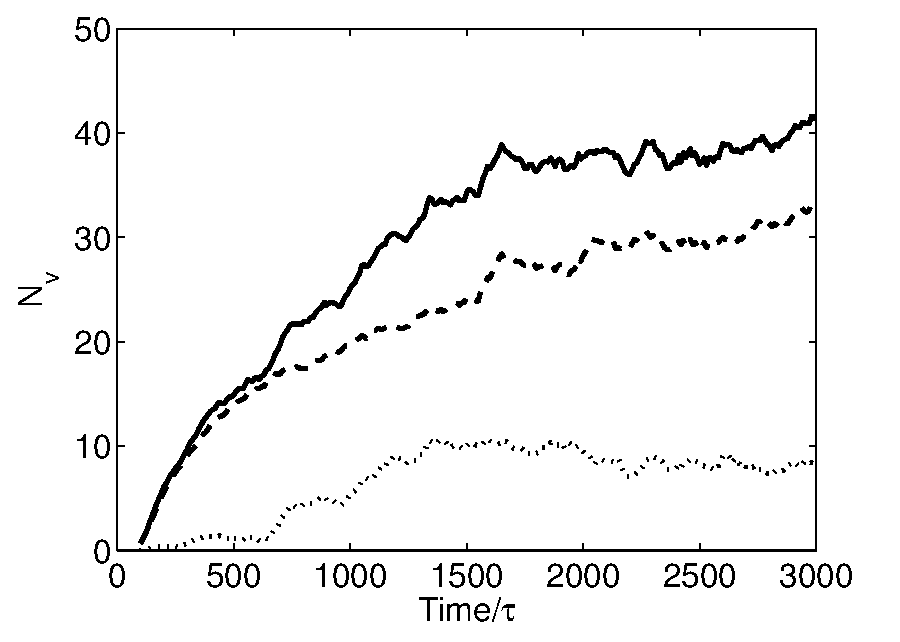
\includegraphics[width=0.45\linewidth]{./afm/figures/nvpn3bw}
%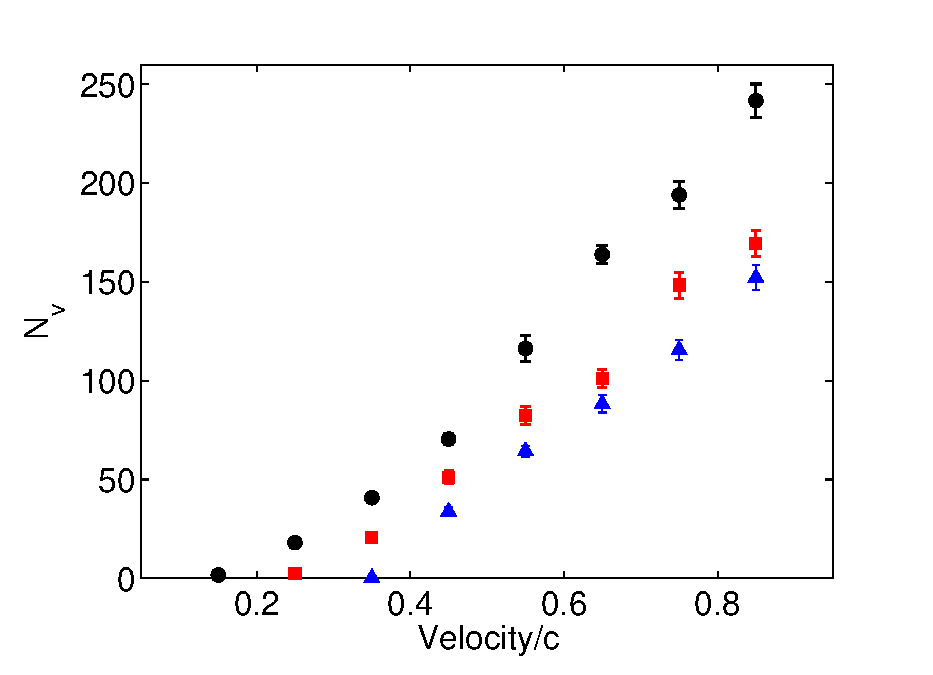
\includegraphics[width=0.45\linewidth]{./afm/figures/nv_v}
%\caption{\label{fig:nvort} (a) Number of vortices produced during $v=0.35c$ flow past the surface.  Shown are the numbers of total %vortices $N_v$ (solid line), positive vortices (dashed line) and negative vortices (dotted line). (b) Final number of vortices $N_v$ as a %function of the flow velocity $v$ for the 2d simulations.  Each data point represents the average of 20 measurements of $N_v$ in the %vicinity of $t=3000\tau$.}
%\end{figure} 

 
\section{Three-dimensional results}
We now move on to focus on the three-dimensional case, modelling the entire 3D surface by utilising the entire AFM data set. Due to the large computation requirements of a fully 3D numerical simulation of the scale required, only the full height surface (no truncation) at only few velocities is studied.

\subsection{Vortex nucleation from the surface}
As with the two-dimensional case, in the vicinity of the surface the local fluid speed, $v=|{\bf v}|$, is enhanced considerably by the surface roughness, with maximum speeds occurring near the tallest mountain. This can be seen through inspection of the local velocities near the surface, shown for several points in time in Figure \ref{fig:velsandvorts} (a-c). Throughtout the simulation the areas of highest velocity occur near the surface prominences seen in Figures \ref{fig:afmsmooth}.

\begin{figure}
  \centering
  \makebox[\textwidth]{
  \begin{minipage}{1.1\textwidth}
  \begin{tikzpicture}
    \begin{axis}[
        width=0.33\linewidth,
        xlabel={\phantom{$x/\xi$}},
        ylabel=$y/\xi$,
        xmin=-180,
    xmax=180,
    ymin=-180,
    ymax=180,
        major tick length = 0.07cm,
        axis on top,
      major tick length = 0.07cm,
      unit vector ratio=1 1 1,
      ]
      \addplot graphics [xmin=-180,xmax=180,ymin=-180,ymax=180] {afm/vels1.png};
    \end{axis}
  \end{tikzpicture}
   \begin{tikzpicture}
    \begin{axis}[
        width=0.33\linewidth,
        xlabel={$x/\xi$},
        ylabel={},
        xmin=-180,
    xmax=180,
    ymin=-180,
    ymax=180,
        major tick length = 0.07cm,
        axis on top,
      major tick length = 0.07cm,
      unit vector ratio=1 1 1,
      ]
      \addplot graphics [xmin=-180,xmax=180,ymin=-180,ymax=180] {afm/vels2.png};
    \end{axis}
  \end{tikzpicture}
   \begin{tikzpicture}
    \begin{axis}[
        width=0.33\linewidth,
        xlabel={\phantom{$x/\xi$}},
        ylabel={},
        xmin=-180,
    xmax=180,
    ymin=-180,
    ymax=180,
        major tick length = 0.07cm,
        axis on top,
        colorbar style={title={$v/c$},text width=0.5em,major tick length = 0.07cm},
      major tick length = 0.07cm,
      point meta min = 0,
      point meta max = 1.6,
      unit vector ratio=1 1 1,
      colorbar,colormap name=invmathot
      ]
      \addplot graphics [xmin=-180,xmax=180,ymin=-180,ymax=180] {afm/vels3.png};
    \end{axis}
  \end{tikzpicture}\\
  \hspace*{0.02\linewidth}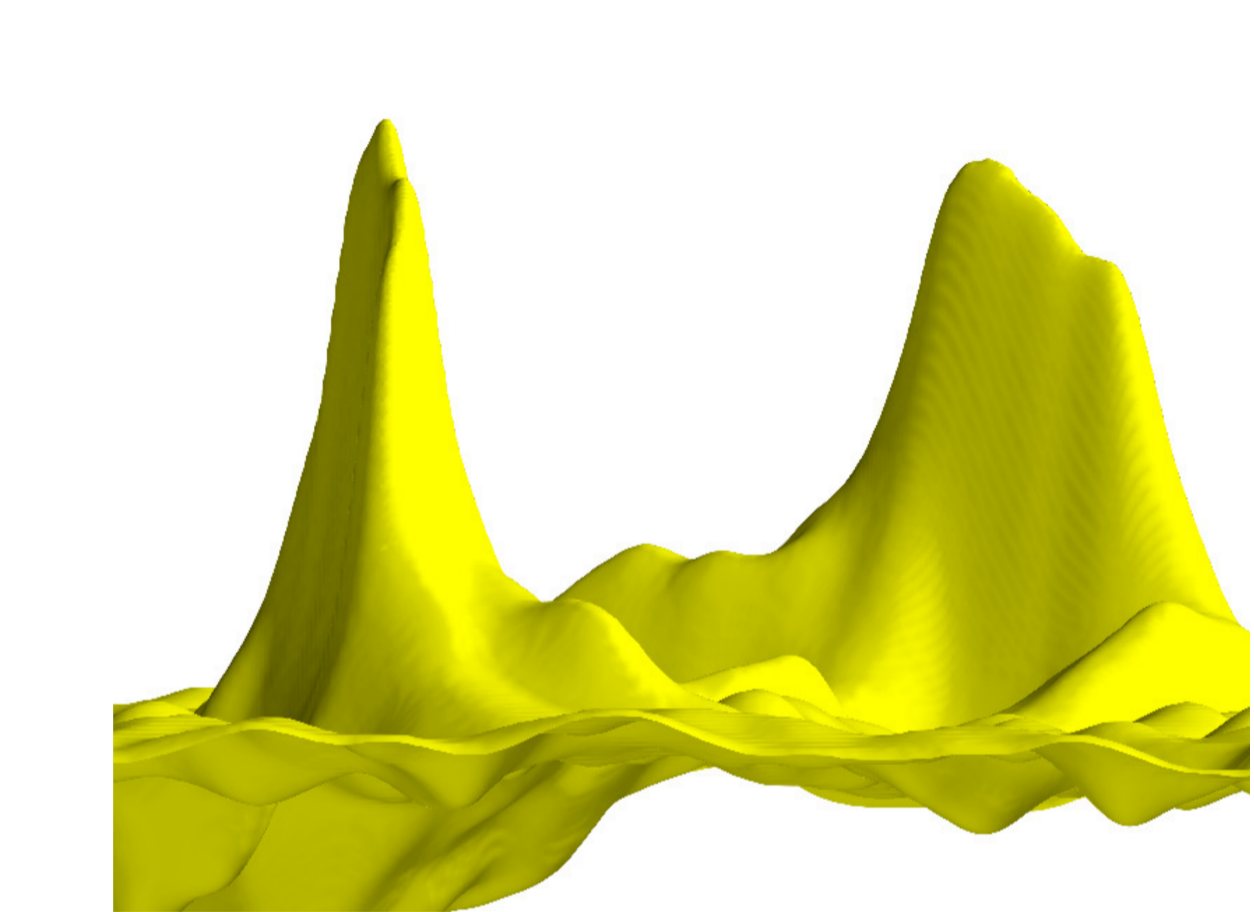
\includegraphics[width=0.3\linewidth]{./afm/afm-sub-2102}
  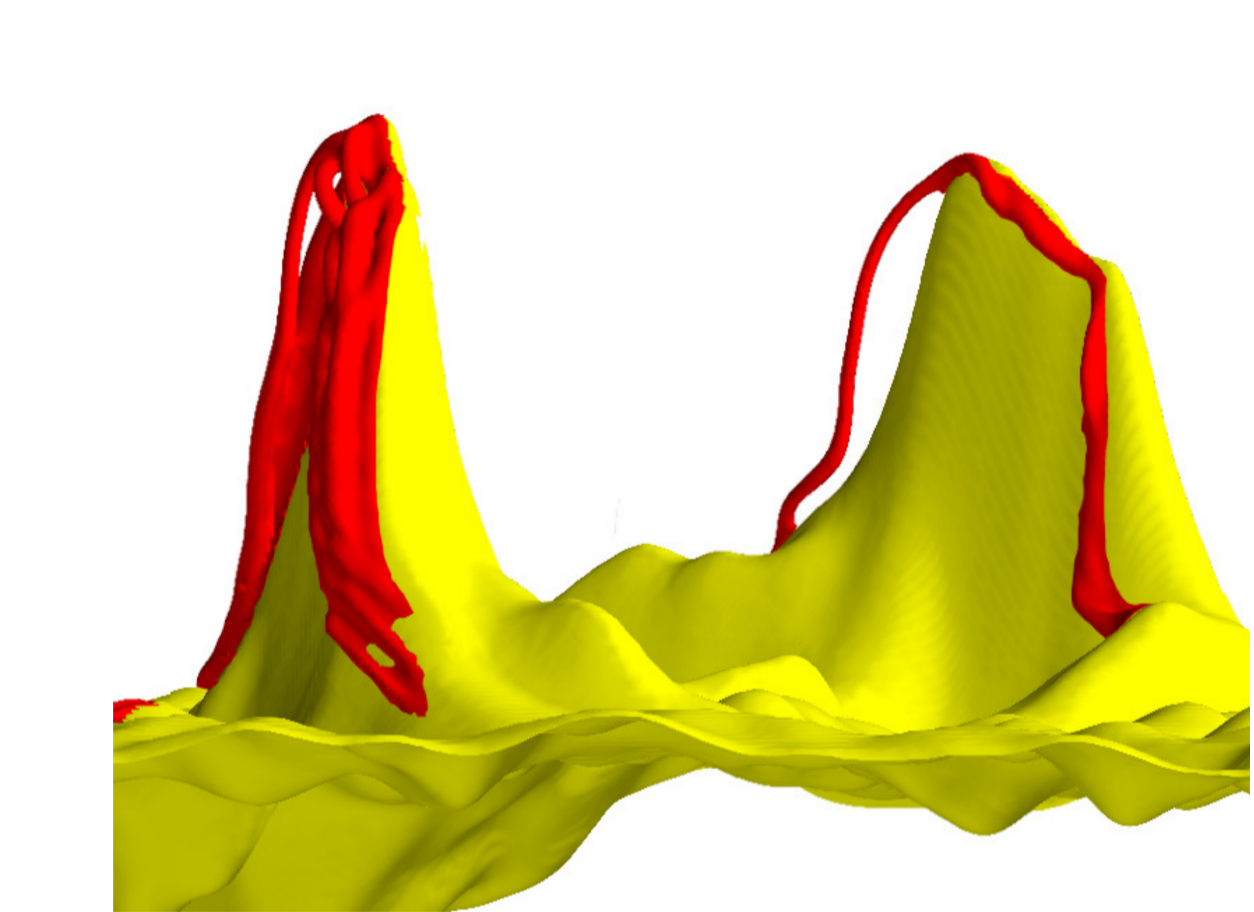
\includegraphics[width=0.3\linewidth]{./afm/afm-sub-3101}
  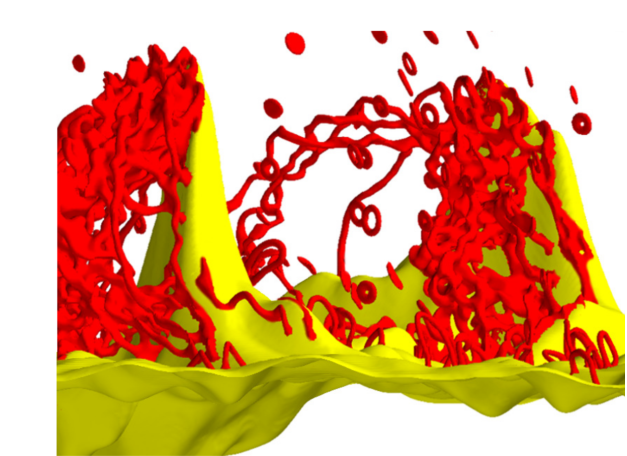
\includegraphics[width=0.3\linewidth]{./afm/afm-sub-10101}
  \end{minipage}
  }
  \caption{\label{fig:velsandvorts}(Upper) Magnitude of the local fluid speed, $v=|{\bf v}|$, shown in the $xy$-plane and computed just above the surface (where the
density drops to $n=0.1 \rho$), at three times $t=20,30,100\,\tau$.  (Lower) Zoomed-up density isosurface plots of density $n({\bf r},t)$ (plotted at 25\%  of the bulk density), showing the surface (yellow) and vortices (red) in the vicinity of the two tallest mountains (view taken along $y$ over the $x$-range $15 \xi \leq x \leq 125 \xi$) at the same times.  %Just prior to vortex nucleation [(left) $t=20 \tau$], the largest fluid speed arises in the vicinity of the highest mountains.  When the fluid speed becomes supercritical at the highest mountains [(middle)$t=30 \tau$], vortex lines becomes nucleated.  At later times [(right)$t=100 \tau$], vortices continue to be shed predominantly by the highest mountains, where the fluid speed continues to be highest.  
%The nucleation vortex loops pass downstream (to the left of the mountains), filling a turbulent layer up to the height of the highest mountain.  This causes a marked downstream spreading of high fluid speed. }
}
 \end{figure} 

As expected, up to a critical imposed velocity, the flow remains laminar and free of vortices.  The critical velocity for vortex nucleation across this particular surface occurs for an imposed flow of $v_c\approx 0.2 c$; this is considerably smaller than, say a hemispherical bump for which $v_c \approx 0.5 c$ \cite{win01},  indicating the significant role of the surface roughness in enhancing the breakdown of laminar flow, similarly to the two-dimensional case. For an increased imposed flow velocity of $u=0.6\,c$, the critical velocity is first exceeded at the highest mountain, leading to nucleation of vortex lines, shown in Figure \ref{fig:velsandvorts} (e), and then by other high mountains on the surface.

Nucleated vortices either peel off the boundary, or, more frequently, slide
down the slopes of the mountains in the form of partially attached vortex loops (carried by the imposed flow). Similarly to the 2D case, vortex loops are nucleated of the same circulation and form vortex clusters (manifesting as partially attached vortex bundles in 3D) on the leeward side of the mountains.

The combined velocity field of the vortex bundles along with nucleation of small vortex loops throughout the surface causes an increase and spreading of areas with high local velocity near the surface, visible in Figures~\ref{fig:velsandvorts}(b, c). The velocity field causes vortex stretching and further vortex nucleation, distorting the organised bundles of vortices and small rings into a complex tangle downstream of the mountains. The resulting tangle is continuously fed by further vortices nucleated from the surface. Vortex bundles and the beginnings of such a tangle can be seen in Figure \ref{fig:velsandvorts}(f). The fully developed vortex tangle in the vicinity of the surface is demonstrated in Figure \ref{fig2}.

\subsection{Three-dimensional boundary layer}
\begin{figure}
\centering
\raisebox{0.8cm}{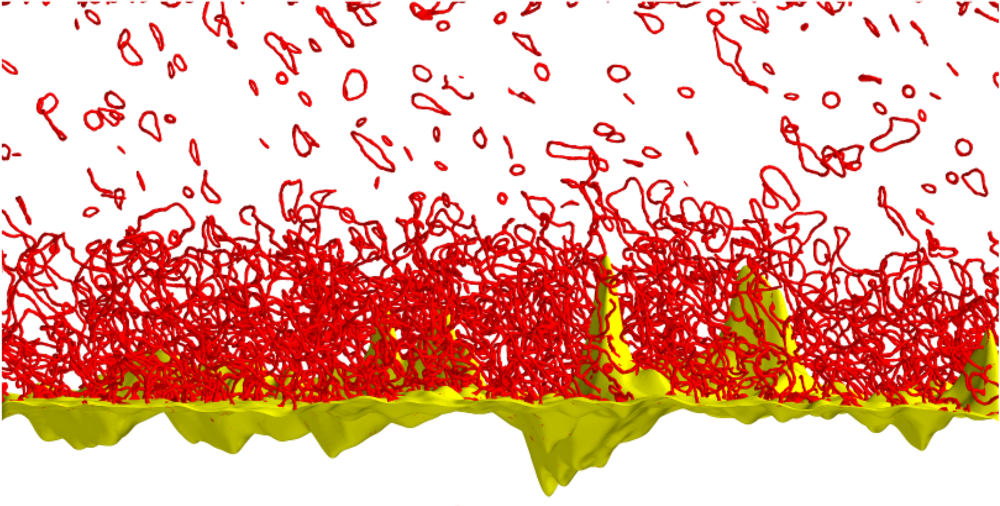
\includegraphics[width=0.5\linewidth]{./afm/fig2-2a}}%
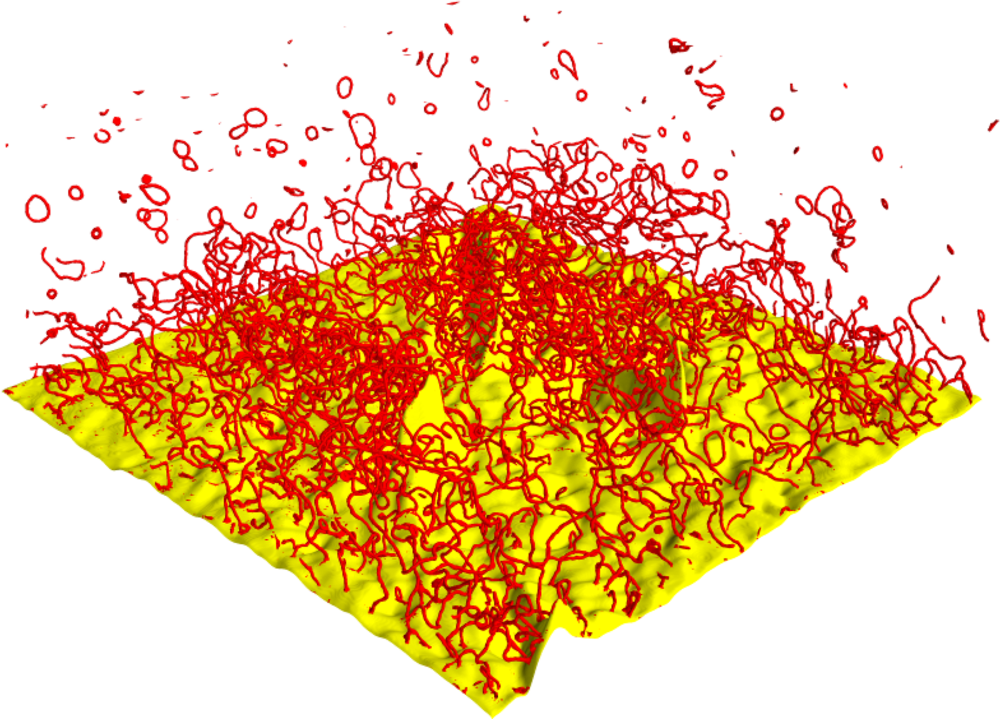
\includegraphics[width=0.5\linewidth]{./afm/fig2-2b}%
\caption{Instantaneous isosurfaces of density $n({\bf r},t)$ 
(plotted at 25\%  of the bulk density) showing the surface (yellow) and vortices (red) for a super-critical flow ($u=0.6 c$) in the saturated 
turbulent regime reached at long times ($t=1220 \tau$).  Notice the turbulent boundary layer up to
approximately the height of the highest mountains and the region
of small vortex rings above it.}
\label{fig2}
\end{figure}
We focus on our 3D simulation with an imposed flow speed of $u=0.6\,c$. For this combination of surface and flow speed, as the number of vortices increases the complex turbulent region of vortex loops and rings remains strongly localised to the vicinity of the surface, up to approximately the height of the highest mountain. The localised region of vortex lines can be seen to form a distinct layer, visible in the lower half of Figure \ref{fig2} (a). In addition to the boundary layer, reconnections due to the interaction of neighbouring vortex lines causes a continuous ejection of vortex rings which spread into the bulk, visible in
the upper part of Figure \ref{fig2} (a-b).

As the layer forms, the vortex line-length in the vicinity of the boundary increases with time at a much faster rate than in the bulk. However, once the layer has covered the entire computational surface, the vortex line-length within the boundary layer approximately saturates. Vortex rings are continued to be ejected from the layer, and so the vortex line length in the bulk continues to slowly grow. For the slower, but still super-critical, imposed flow with speed $u=0.2\,c$ the turbulent layer still forms with the same height, albeit with reduced density of vortices, generalising the behaviour of the boundary layers that formed in our 2D simulations.

The turbulent layer and ejected vortex rings are not isotropic: on average, vortex lines are flattened parallel to plane of the surface and the ejected vortex rings lie more in the $xy$ plane (so that they travel vertically away from the layer).

\subsubsection{Vortex line-length density}
\begin{figure}
  \centering
  \begin{tikzpicture}
    \begin{axis}[ylabel near ticks,xlabel near ticks,
        width=0.6\linewidth,
        height=0.4\linewidth,
        xlabel={$t/\tau$},
        ylabel={$L_{0}$ \& $L_{1}$},
        xmin=0,
        xmax=1300,
        ymin=0,
        xtick pos=left,
        ytick pos=left,
        major tick length = 0.07cm,
        axis on top
      ]
      \addplot[mark=*,thick,blue,line join=round] table[x=t,y=top]{afm/vv_t.dat};
      \addplot[mark=square*,thick,red,line join=round] table[x=t,y=bot]{afm/vv_t.dat};
    \end{axis}
  \end{tikzpicture}
  \caption{\label{fig:vortlinedensdt}Vortex line-density below ($L_0$, red squares) and above ($L_1$, blue circles) the height of $z=100\xi$, approximately the height of the tallest mountain, for a 3D simulation with imposed flow speed of $u=0.6\,c$.} 
  \end{figure}
We monitor vortex line-density below and above the height of the highest mountain $L_0$ and $L_1$ respectively. By measuring line-density in this way we are able to ascertain two things. Firstly, we will be able to measure if the boundary layer's vortex density over time, so as to say when the layer has saturated. Secondly, we can compare values in the region of the surface and away from the surface, as a measure of the strength of the boundary layer. We split the computational box in half, for $z<100\xi$ and $z \geq 100\xi$. We then estimate the vortex line-length using the vortex cross sectional area, $A$ and the volume of the isosurface tubes in each half of the computational box, obtaining vortex line-length $V_0(t)/A$ and $V_1(t)/A$. Finally these two quantities are used to compute the vortex line-densities throughout the simulation, shown in Figure \ref{fig:vortlinedensdt}.

We find that both $L_0$ and $L_1$ grow over time as vortex lines are nucleated into the superfluid. $L_0$ saturates at a value around $1.2\times 10^{-4}$ at $t \approx 800$, confirming the growth of vortex line-density up to saturation in the lower region of the computational box. On the other hand, $L_1$ grows much slower than $L_0$ and shows significantly less vortex line-density throughout the simulation, and does not saturate but instead exhibits a steady growth of vortex line-length throughout, even after $L_0$ has saturated at $t \approx 800$.

These measurements show a transient period of vortex line-density growth at early times which saturates into a boundary layer in the lower half of the computational box, corresponding to the region in the vicinity of the rough surface prominences. In addition, we have quantified a continuous process of vortex ring formation and emission into the upper half of the computational box, corresponding to the bulk of the superfluid. This process is further investigated in Section \ref{sec:vortexmill}.

\subsubsection{Velocity profile}
\begin{figure}
  \centering
  \begin{tikzpicture}
   \begin{axis}[ylabel near ticks,xlabel near ticks,
        width=0.5\linewidth,
        height=0.5\linewidth,
        xlabel=$x/\xi$,
        ylabel=$\phantom{y/\xi}$,
        xtick pos=right,
        ytick pos=right,
        yticklabels={,,},
        ytick={},
        xmin=-180,
        xmax=180,
        ymin=0,
        ymax=195,
        major tick length = 0.07cm,
        axis on top,
      ]
      \addplot graphics [xmin=-200,xmax=200,ymin=0,ymax=98] {afm/shadow.png};
    \end{axis}
    \begin{axis}[ylabel near ticks,xlabel near ticks,
        width=0.5\linewidth,
        height=0.5\linewidth,
        xlabel={$v_{\rm xy}/c$},
        ylabel={$z/\xi$},
        xmin=0,
        xmax=0.8,
        ymin=0,
        ymax=195,
        xtick pos=left,
        ytick pos=left,
        major tick length = 0.07cm,
        axis on top
      ]
      \addplot[mark=none,ultra thick,blue,line join=round] file {afm/vels_z.dat};
    \end{axis}
  \end{tikzpicture}
  \caption{Typical local flow speed (lower abscissa) at various heights above the surface of the wire, averaged over $10$ points in time, at $1130<t/\tau<1220$. For comparison, a 2D sample of the 3D surface ($y=0.1\,\mu$m, demonstrating one of the tallest surface features) is shown in grey (upper abscissa).} 
  \end{figure}
We further explore the turbulent boundary layer by measuring the local velocity as a function of distance, so as to obtain a velocity profile. We measure the quantity 
\begin{equation}
  v_{\rm xy}(z) = \langle v(x,y,z) \rangle_{\rm xy},
\end{equation}
where $\langle v(x,y,z) \rangle_{\rm xy}$ denotes averaging of the fluid velocity in the $xy$ plane and $v=|\bf {v}$|. We measure $v_{\rm xy}(z)$ at 10 snapshots for times $1130<t/\tau<1220$, so that the vortex line-length in the vicinity of the surface is saturated. The resulting quantity $v_{\rm xy}(z)$ is a measurement of the typical local speed of the fluid flow at the height of $z$.

We find that for the simulation with $u=0.6\,c$, the fluid velocity far away from the surface is unaffected by the rough surface. The typical local velocity is equal to the imposed flow velocity. The speed of the flow is $v_{\rm xy}(z)\approx0.6$ for all $z \lesssim 100\xi$, the approximate height of the highest prominence. In the region $40 \lesssim z \lesssim 100\xi$ the overall effect of the vortices in that region is to counteract the imposed flow velocity. The overall effect is that the typical flow speed is slower the closer to the surface it is measured, in analogy to a viscous boundary layer in classical fluids. In the region $0 \lesssim z \lesssim 40\xi$ most of the computational volume is now below the surface, and so only the fluid in the valleys of the surface is computed as part of the average. In this region the typical speed of the flow rapidly drops to almost zero.

\subsection{\label{sec:vortexmill}Vortex ring generation through the vortex mill mechanism}
At early times, nucleated vortex lines can form aligned along the flow direction, twisted due to the bundling of vortex lines nucleated at high-frequency. An example of this structure can be seen in the background of Figure \ref{fig:velsandvorts} (f). The twisted vortex lines generate more vorticity feeding into the boundary layer tangle, by spooling small vortex loops though the vortex-mill mechanism envisaged by Schwarz \cite{PhysRevLett.64.1130}. This confirms that, for the AFM surface and an imposed flow of $u=0.6\,c$, the vortex tangle which develops can be interpreted as generated either intrinsically or extrinsically: in both cases vortices nucleate at the highest mountains before filling the layer below.

At later times (due to the modified velocity field by the saturated boundary layer) and for higher imposed flow velocities, the critical velocity is exceeded across greater areas of the surface. However, even after the generation of a considerable vortex tangle, the highest mountains continue to dominate vortex nucleation; here the fluid velocity is always the highest and vortex shedding occurs at the fastest rate. Despite this, we have already seen that the vortex line-density in the lower half of the computational box (corresponding to the fluid in the vicinity of the surface roughness) remains saturated. To maintain equilibrium, vortex line-length is constantly ejected from the boundary layer by the process of twisting, vortex reconnections, and the formation of vortex rings that detach and fly in the positive $z$ direction. An example of this process is seen in Figure ... ,demonstrating a further vortex mill mechanism, where vortex line-length is injected into the bulk of the superfluid in the form of escaping rings.

\begin{figure}
\centering
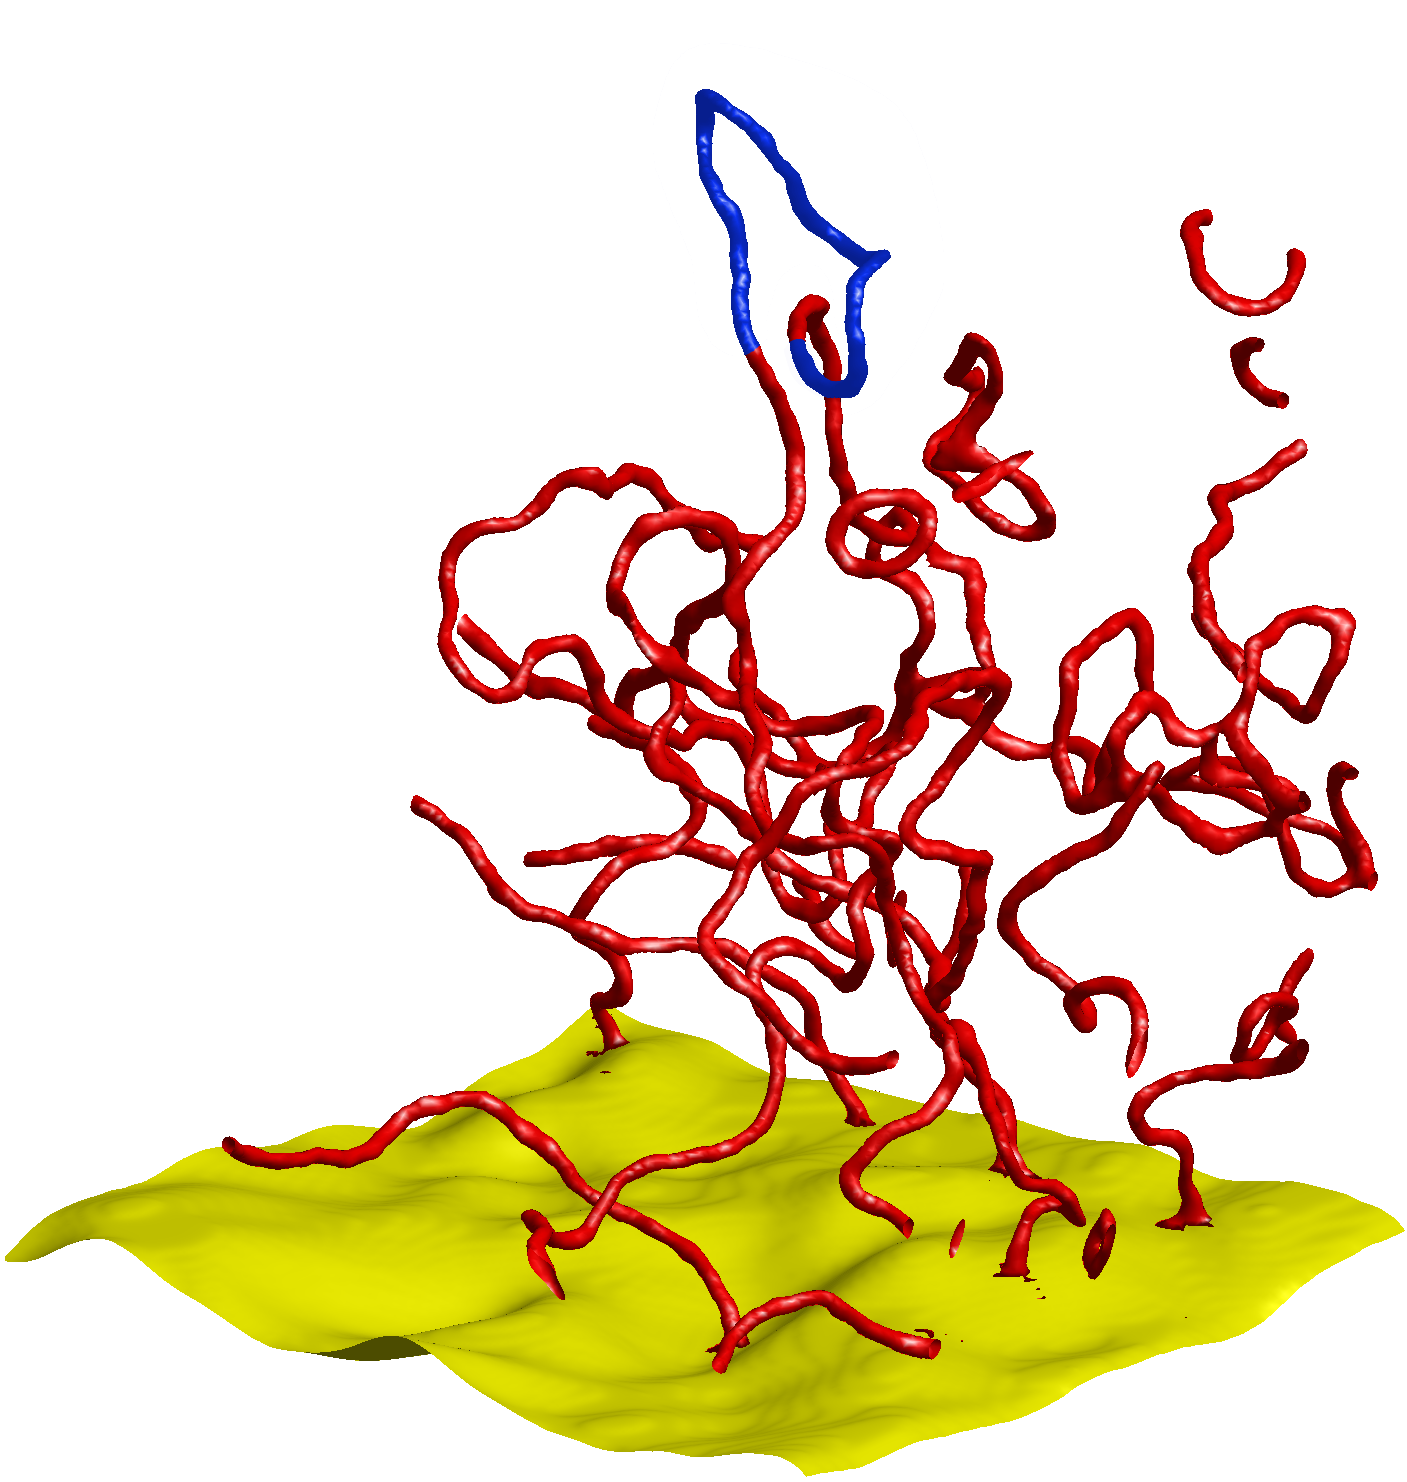
\includegraphics[width=0.25\linewidth]{./afm/mill1}%
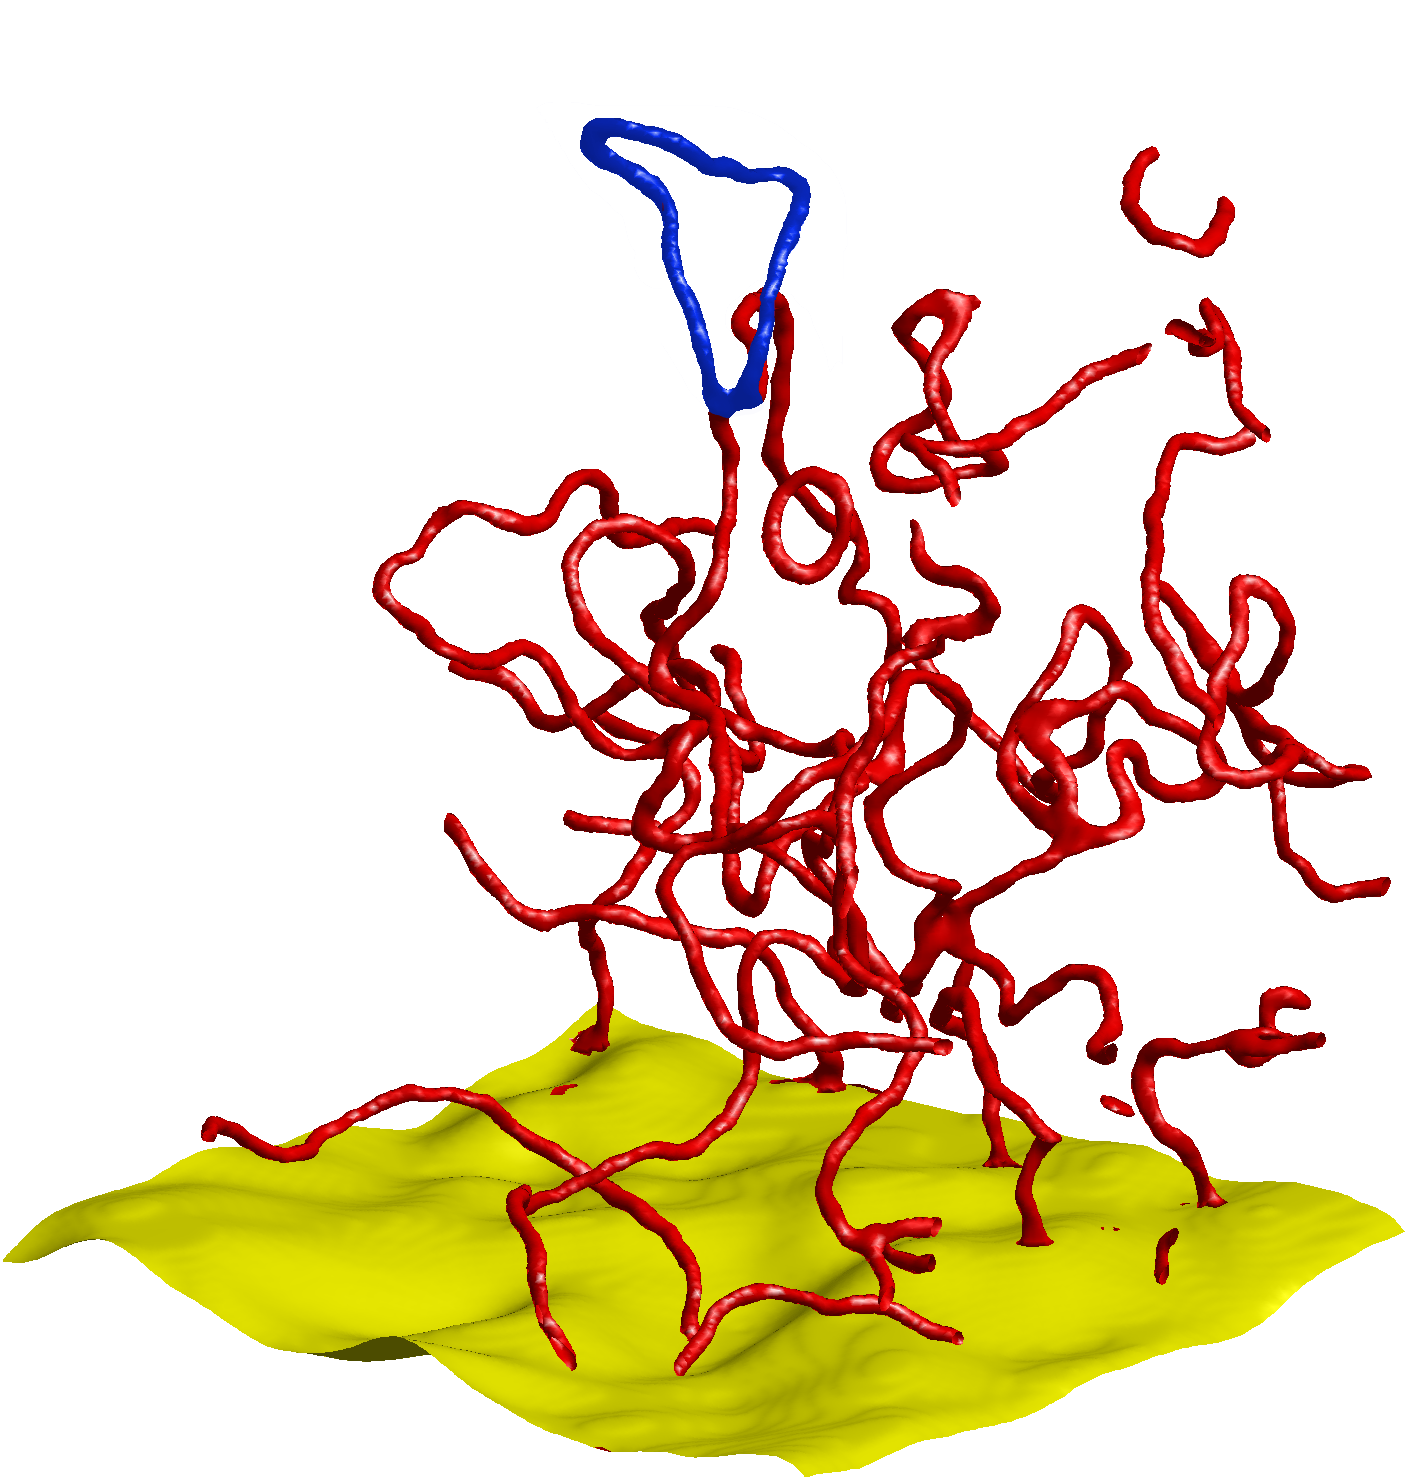
\includegraphics[width=0.25\linewidth]{./afm/mill2}%
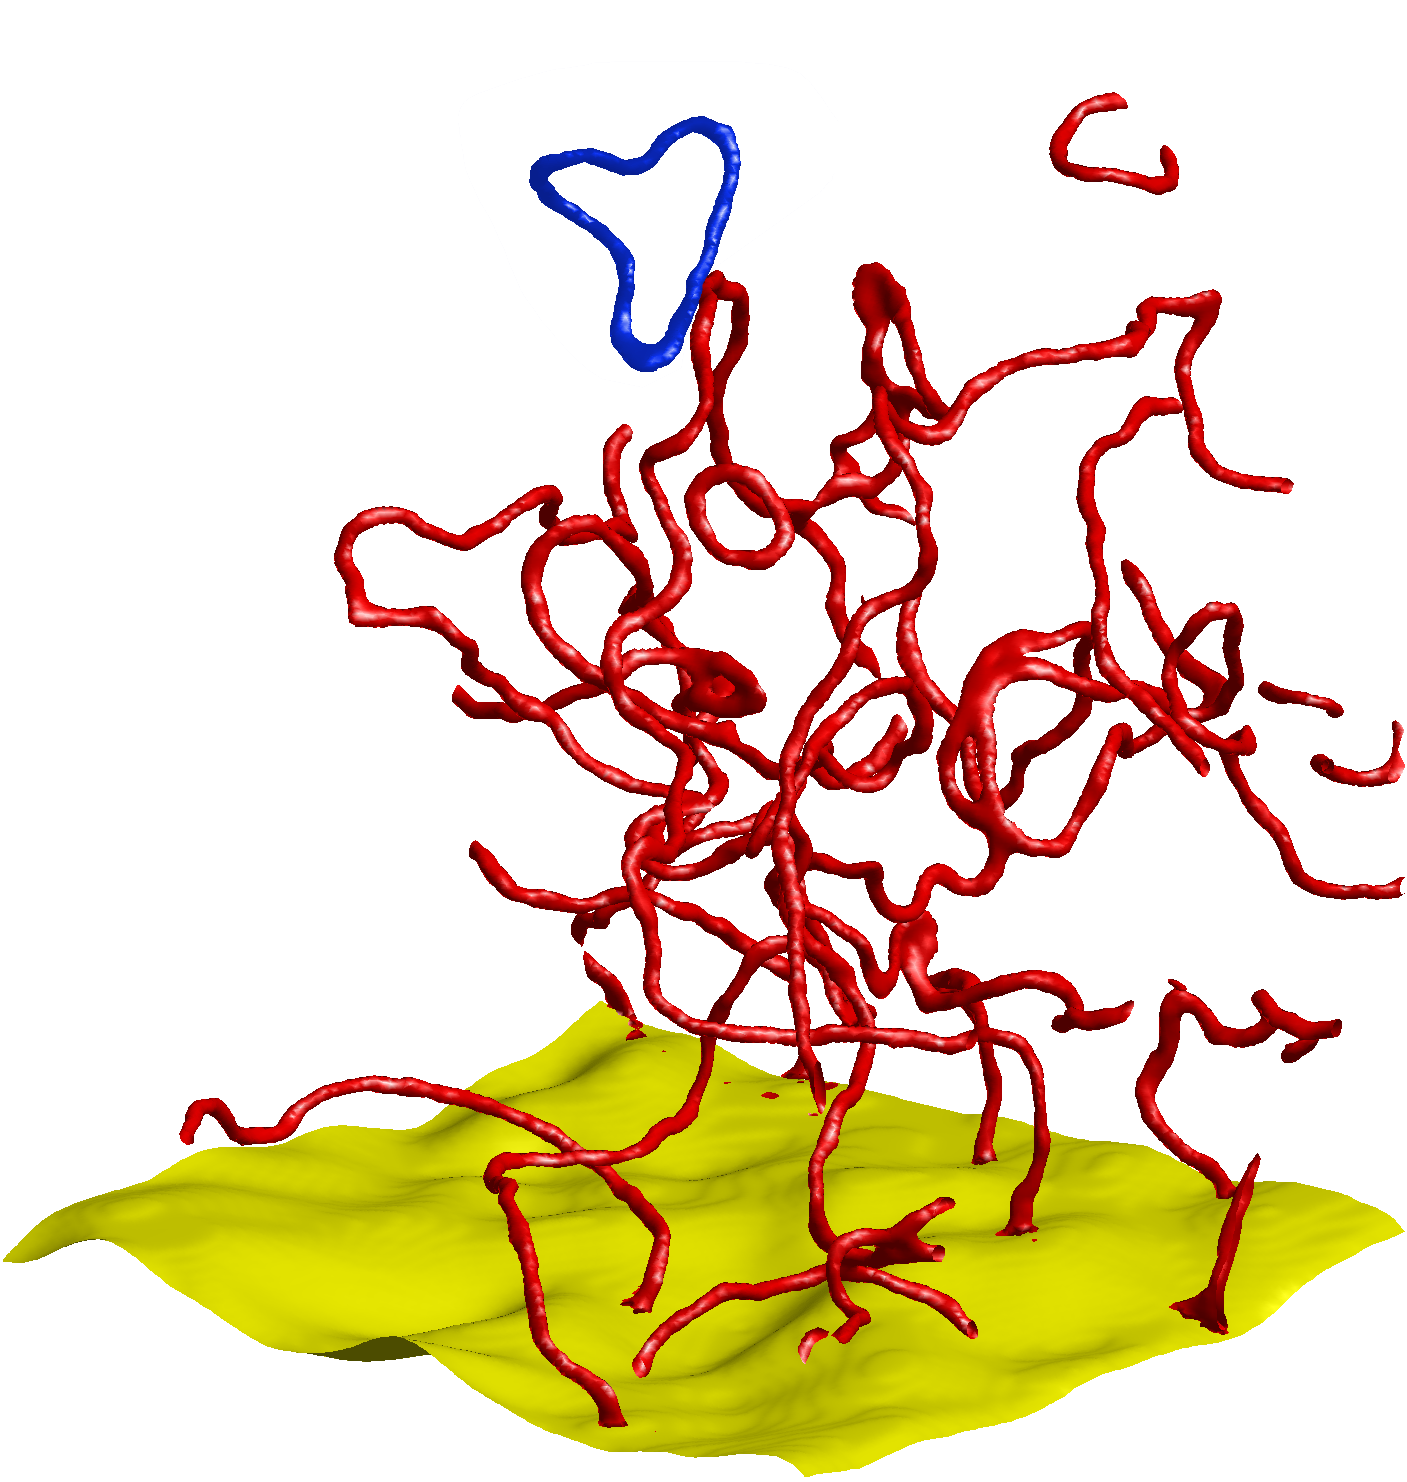
\includegraphics[width=0.25\linewidth]{./afm/mill3}%
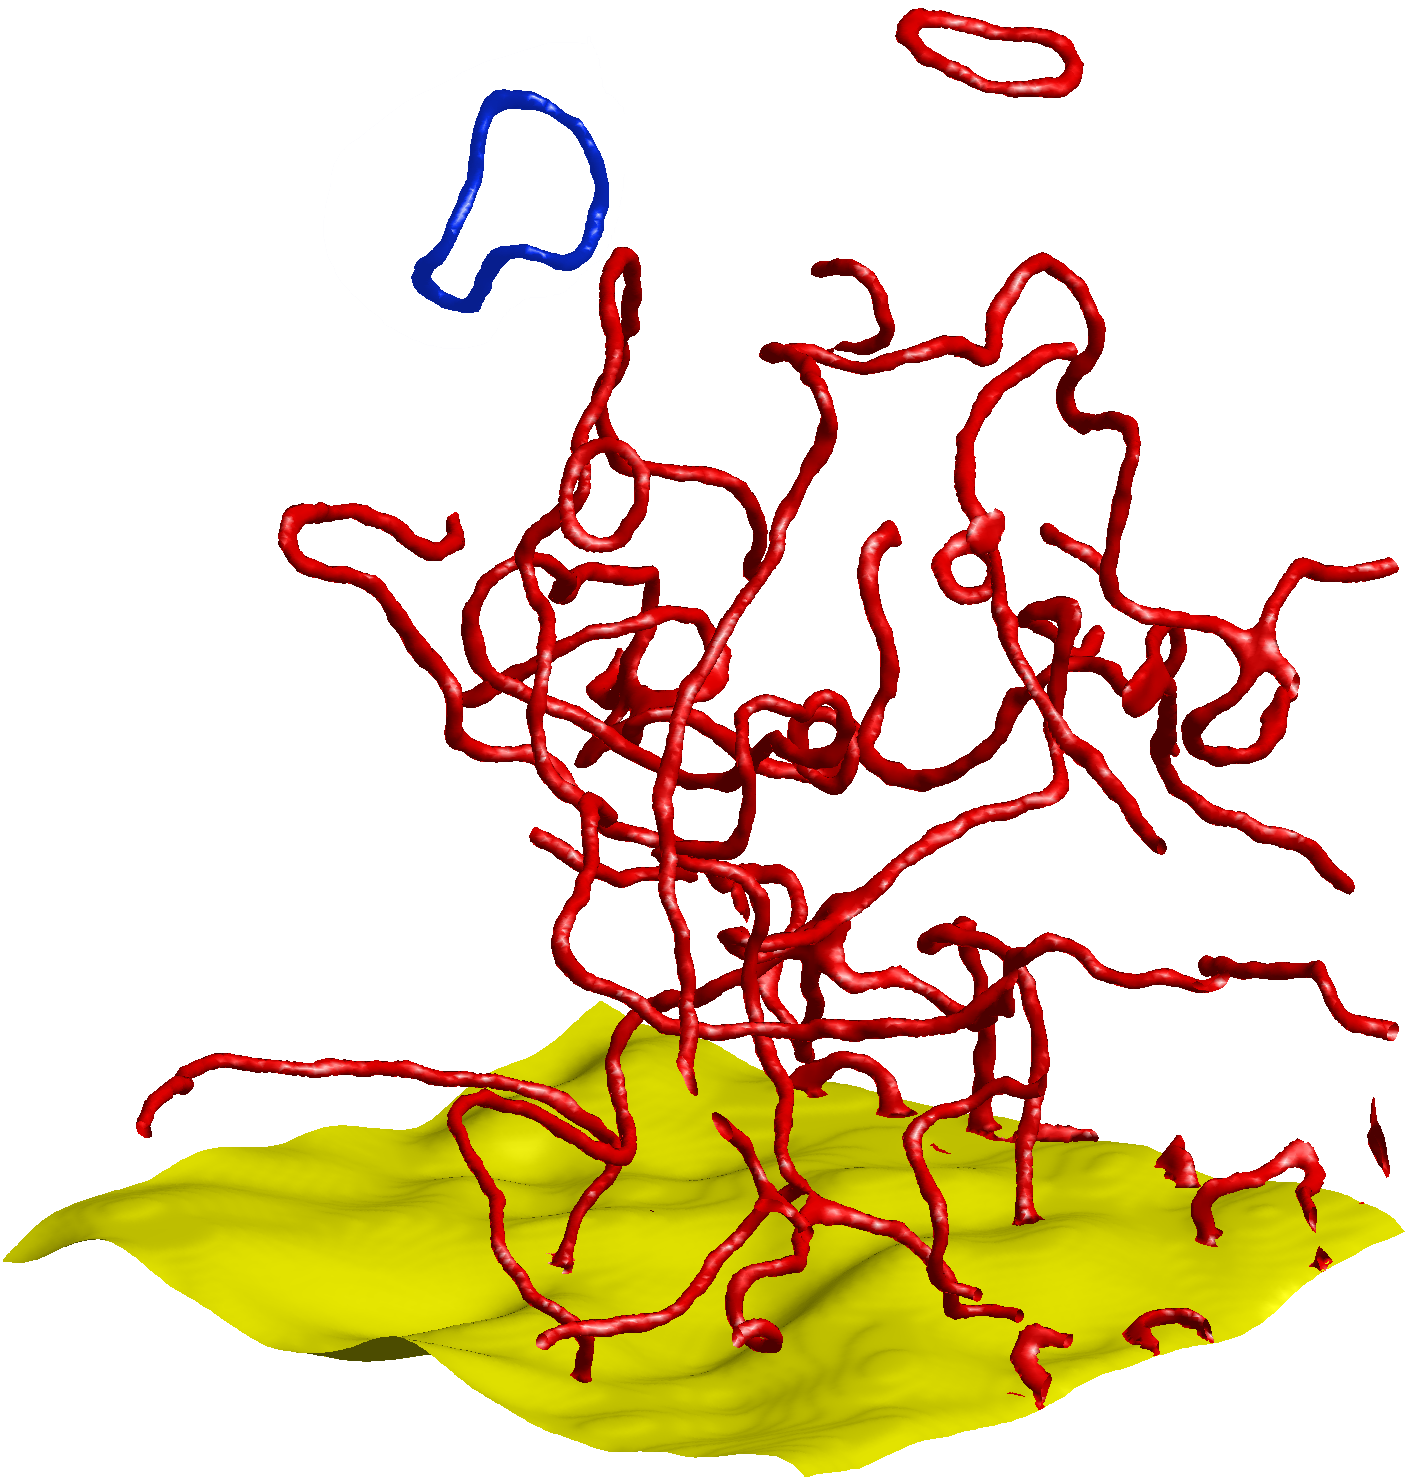
\includegraphics[width=0.25\linewidth]{./afm/mill4}%
\caption{Instantaneous isosurfaces of density $n({\bf r},t)$ 
(plotted at 25\%  of the bulk density) showing the surface (yellow) and vortices (red) for the flow ($u=0.6\,c$) in the saturated turbulent regime reached at long times ($t/\tau=730,740,750,770$). Demonstrated in blue is an escaping vortex ring (originating in the tangle and formed due to the vortex mill mechanism) that travels in the positive $x$ direction, into the bulk of the fluid.}
\label{fig:escapering}
\end{figure}


\section{Conclusions}

The experimental implications of `superfluid boundary layers` on macroscopic
observables need to be investigated.  Our results should
particularly stimulate experiments in $^3$He-B, where, due to relative
large healing length, it is possible to study flows with controlled 
surface height roughness. 

\end{chapter}


%\section{\label{section:sfwire} Superfluid wire experiments}
%Developments in flow visualization at very low temperatures
%\cite{Guo2014,Fisher2014} have
%driven recent progress in the turbulence in superfluid $^4$He and
%$^3$He-B. Experiments and theory have highlighted effects
%such the existence of classical and
%nonclassical turbulent regimes \cite{WalmsleyGolov2008}, and
%energy transfer over length scales, both
%direct \cite{Barenghi2014} and inverse
%\cite{WalmsleyTompsett2013,Baggaley2014}.
%At the same time, improvements in the generation, observation and control of quantum
%vortices in atomic Bose--Einstein condensates\cite{Henn,Freilich2010,aioi11,neely_bradley_13,kwon_moon_14}
%has added a character of interdisclinarity to the study of
%turbulence in quantum fluids.

%In many superfluid helium experiments \cite{VinenSkrbek2008}, turbulence
%is generated by moving grids \cite{Davis2000},
%wires \cite{Guenault1986,brad05,Bradley2011,Fisher2001,goto08},
%forks \cite{Blaauwgeers2007,Bradley2012} or spheres \cite{Schoepe1995}.
%Although macroscopically polished, the surface of these objects is
%rough on the length scale of the superfluid vortex core, which is of
%the order of $10^{-10}~\rm m$ in $^4$He
%and $10^{-8}~\rm m$ in $^3$He.  As an example, Fig.~\ref{fig:afmimg}(a) is an atomic force microscope (AFM) image showing the microscopic detail on the surface of a  single--core NbTi `floppy' wire used for generating superfluid turbulence  \cite{Bradley2011}.  Note the appearance of an elongated scratch, typical of such wires.  No direct flow visualization is available on these microscopic length scales and, as such, 
%superflow in the presence of walls remains poorly understood. In principle, the superfluid boundary conditions should
%be straighforward.
% the simplest case of a boundary at rest, the superfluid velocity
%component which is perpendicular to the boundary must be equal to
%zero at the boundary, while the tangential component can slip.
%In practice, nucleation of quantum vorticity complicates
%this idealized Eulerian picture.

%The established theoretical approaches used to successfully describe
%homogeneous superfluid turbulence away from boundaries can falter in the presence of realistic boundaries.
%First consider the vortex filament method of Schwarz
%\cite{Schwarz,Hanninen-PNAS}. Its application to relatively simple and smooth
%boundaries, such as spheres \cite{Hanninen-sphere,Kivotides-sphere} and
%hemispheres \cite{Schwarz-bump}, has proved
%cumbersome due to the complex system of images which is required.
%Its starting assumption, that the vortex core
%is infinitesimally smaller than any other length scale, makes it
%unsuitable for realistic boundaries of roughness comparable to
%the vortex core size.  Moreover Schwarz's approach requires arbitrarily seeding
%vortex loops, because it does not account for vortex nucleation.
%Another approach which suffers similar difficulties \cite{Henderson} is
%the two--fluid Hall--Vinen--Bekarevich--Khalatnikov (HVBK)
%equations \cite{Salort2011,Salort2012}. Moreover, the HVBK equations are coarse--grained over
%length scales larger than the average vortex separation, hence the
%boundary conditions require further assumptions or the introduction of
%unknown sliding/pinning parameters.

%A practical dynamical model of superflow near boundaries of arbitrary
%shape which is powerful enough to describe vortex nucleation is
%the Gross--Pitaevskii equation (GPE) \cite{RobertsBerloff}.  While the GPE is an accurate quantitative description of atomic condensates, it provides only a qualitative model of superfluid helium.  Frisch {\it et al.} pioneered the GPE approach by simulating superflow past a cylinder, observing vortex pair nucleation above a critical flow speed \cite{frisch92}.  Subsequent GPE-based works have further elucidated vortex generation past a cylinder \cite{nore93,jma99,saito10}, as well as spheres and half-spheres \cite{winiecki99}, and elliptical objects \cite{stagg_parker_14}.    Nevertheless, at this stage of investigation, the GPE is the optimum tool 
%to gain physical insight into the flow of a superfluid over
%rough surfaces typical of experiments.

%Our numerical approach is to first obtain the stationary solution for the static fluid $(v=0)$, achieved via imaginary time propagation of the GPE \cite{Minguzzi2004}.  From this initial condition the GPE is then propagated in real time, with the fluid speed $v$ ramped up smoothly from zero up to its required value.